\chapter{O-minimal Geometry}
\section{Overview}

O-minimal geometry was developed in the 1980s by various authors
including Pillai, Steinhorn, and van den Dries. Some call it an
incarnation of Grothendieck's vision of a ``tame topology'' described
in his ``Esquisse d'un Programme''. It strives to generalize real
semi-algebraic geometry to include also real (sub)-analytic sets.
This makes it a powerful and robuts tool to study various problems
including conjectures in diophantine geometry.

O-minimal Geometry has strong ties mathematical logic and model
theory. 

The basic motivation is to carve out a class ``interesting'' subsets
of $\IR^n$ that is stable under various basic observations. These sets
will be called ``definable'' (in a given o-minimal structure). 

For example, consider an algebraic curve $C\subset (\IC^\times)$ and
the map $\be \colon\IR^2\rightarrow (\IC^\times)^2$ defined by
\begin{equation*}
  \be(x,y) = (e^{2\pi i x},e^{2\pi i y}). 
\end{equation*}
Consider the set $X = \be^{-1}(C) \cap [0,1)^2$. Then $C$ contains
infinitely many torsion points of $(\IC^\times)^2$ if and only if $X$
contains infinitely many rational points.
We will see that $X$ is definable in a certain o-minimal structure.
Note that $X$ is not necessarily real analytic (but it is real
semi-analytic). 

\section{O-minimal Structures}


\begin{definition}
  \label{def:structure}
%  For each $m\in \IN_0$ consider the set of all subsets of $\IR^n$.
  A \emph{structure} $\cS$ is a sequence $(S_m)_{m\in\IN_0}$
  where each $S_m$ is a set of subsets of $\IR^m$ with the following
  properties for all $m\in \IN_0$:
  \begin{enumerate}
  \item [(i)] Each $S_m$ is closed under boolean operations,
    \textit{i.e.}, if $X,Y\in S_m$, then $X\cup Y\in S_m$ and
    $\IR^m\ssm X\in S_m$.
  \item[(ii)] If $X\in S_m$, then $\IR\times X\in S_m$ and $X\times
    \IR\in S_m$.
  \item[(iii)] If $X\in S_{m}$ and $\pi\colon
    \IR^{m}\rightarrow\IR^k$ is the projection to $k$ distinct
    coordinates, then 
    $\pi(X)\in S_k$.
  \item[(iv)] All real semi-algebraic subsets of $\IR^m$ are in
    $S_m$.\footnote{A real semi-algebraic subsets of $\IR^m$ is a
      finite union of sets each of which is set of 
      solutions of a finite number of polynomial equalities and
      strict inequalities.}    
  \end{enumerate}
  We say that a subset of  $\IR^m$ is \emph{definable} in $\cS$ if it
  is a member of $S_m$.
\end{definition}

\begin{example} Let us consider the two extremes.
  \begin{enumerate}
  \item [(i)] Set $S_m$ to be the set of all subsets of $\IR^m$ for
    all $m\ge 0$. Then $(S_m)_m$ is a structure. It is useless in this
    context and will play no role
    in what follows.
  \item[(ii)]
    Set $S_m$ to be the set of all real semi-algebraic subsets of $\IR^m$
    for all $m\ge 0$. By definition each $S_m$ is closed under taking
    unions. Moreover, each $S_m$ is closed under taking intersections.    
    Say $X\in S_m$. Let us  verify that $\IR^m \ssm X$. Indeed, by
    closedness under union and intersection we may assume that either 
    \begin{equation*}
      X = f^{-1}(0)=\{ x\in\IR^m : f(x) = 0\}
      \quad\text{or}\quad       X = f^{-1}((0,\infty))=\{ (x)\in\IR^m : f(x) > 0\}
    \end{equation*}
    for a single $f\in\IR[X_1,\ldots,X_m]$. In the first case
    we have $\IR\ssm X=\{x\in\IR^m : f(x)^2 > 0\}$ and in the second
    case
    $\IR\ssm X = \{x\in\IR^m : f(x)=0\} \cup \{x\in \IR^m: -f(x)^2 >
    0\}$; both are real semi-algebraic.
    Property (ii) in the definition of structure can be verified
    directly. Property (iii) is also true, but harder to show. It
    is called the Seidenberg--Tarski Theorem.
  \end{enumerate}
\end{example}



\begin{exercise}
  Find and understand a proof of Seidenberg--Tarski Theorem. For
  example, one can be found in Chapter 2, \S 2~\cite{D:oMin}. This
  proof runs via a cell-decomposition, a concept we will discuss
  further down. 
\end{exercise}

Here are some direct consequences of the definition of a structure.  

\begin{lemma}
  \label{lem:structprops}
  Let $\cS$ be a structure. Let $X\subset\IR^m$ and $Y\subset\IR^n$ be definable subsets of $\cS$.
  \begin{enumerate}   
  \item [(i)] Then $X\times Y$ is definable.
  \item[(ii)] If $m=n$, then $X\cap Y$ is definable.
  \item[(iii)] The image of $X$ under any polynomial map
    $\IR^m\rightarrow \IR^n$ is definable.
  \end{enumerate}
\end{lemma}
\begin{proof}
  For (i) note that $X\times Y =  (X\times \IR^n)\cap (\IR^m\times
  Y)$. For (ii) we need $X\cap Y = \IR^m\ssm ((\IR^m\ssm X)\cup (\IR^m
  \ssm Y))$.
  Let $p_1,\ldots,p_n\in\IR[X_1,\ldots,X_m]$ and consider the graph
  \begin{equation*}
    \Gamma = \{(x_1,\ldots,x_m,x_{m+1},\ldots,x_{m+n})\in\IR^{m+n} :
    x_{m+i}-p_i(x_1,\ldots,x_m)= 0 \text{ for all }
    i\} 
  \end{equation*}
  of $p=(p_1,\ldots,p_n)\colon \IR^m\rightarrow\IR^n$. Then $\Gamma$ is
  semi-algebraic and it is definable in $\cS$. Now $p(X)$ is the
  projection of $\Gamma \cap (X\times\IR^n)$ to $\IR^n$ and hence also
  definable. This gives (iii). 
\end{proof}

\begin{definition}
  Let $\cS$ be a structure and $X\subset\IR^m$ definable.
  A map $f\colon X\rightarrow\IR^n$ is
  called \emph{definable} in $\cS$, if its graph $\Gamma(f) =
  \{(x,f(x)) : x\in X\}\subset\IR^{m+n}$ is definable.
\end{definition}

Domain $X$ and image $f(X)$ of a definable map must also be definable
by an argument similar to the one in the proof of
Lemma~\ref{lem:structprops}(iii). If $Y\subset \IR^n$ is definable,
then so is the preimage $f^{-1}(Y)$. 

\begin{example}
  Let $\cS$ be an arbitrary structure. 
  On a definable domain, 
  all polynomial functions, all rational functions without poles on the
  domain, and all algebraic functions are definable.
  In particular, $x\mapsto \sqrt{x}$ is definable on $X=[0,\infty)$.
  The absolute value function $x\mapsto |x|$ is definable on $\IR$.
\end{example}



While structures are very flexible, the definition does not contain
any clause that ``tempers'' the collection of sets.

\begin{definition}
  A {structure} $\cS=(S_m)_m$ is call \emph{o-minimal}
  \begin{enumerate}
  \item [(v)]  if each 
  element in $S_1$ is a finite union of points and
  open intervals, that are possibly unbounded.
  \end{enumerate}
\end{definition}

\begin{example}
  By the Seidenberg--Tarski Theorem we already know that the real
  semi-algebraic sets constitute a structure. Say $f\in\IR[X]$.
  The zero locus of $f$ is finite or $\IR$. Moreover,
  $f^{-1}((0,\infty))$ is open in $\IR$ and has only finitely many
  boundary points. So it is a finite union of intervals. Thus this
  structure is o-minimal, we will denote it by $\IRalg$. 
\end{example}

The final axiom (v) in does an excellent job in ``taming'' subsets of
$\IR^m$. This will hopefully be apparent after seeing the
applications. But the axiom comes at a heavy price.
We immediately stake out the limits of o-minimality.

\begin{nonexample}
  Let $\cS$ be an o-minimal structure. Then $\IZ$ is not definable in
  $\cS$. Moreover, the function $\sin \colon\IR\rightarrow\IR$
  is not definable in any o-minimal structure.  
\end{nonexample}
%\begin{definition}
%  Let 
%\end{definition}

\section{Structures and First-Order Logic}

The various sets appearing in Definition~\ref{def:structure}(i) --
(iv) can equivalently be described using first-order logic formulas. In fact, the
terminology ``structure'' comes from mathematical logic. Our main
emphasis will be on the geometry.  But we  take some time to give
an informal overview of the connection to logic as it is equivalent
and often very useful. 

Say $\cS$ is a structure and suppose $X\subset\IR^m$ is definable.
We think of the formula $x\in X$ as an $m$-ary relation signifying
membership of the $m$-tuple $x$ in $X$. Subject to the usual rules we
can combine two formulas using the logical symbols $\wedge$ (for
``and'') and $\vee$ (for ``or''), we can negate them by using $\neg$
(for ``not''), and we may use the existential ($\exists$) and
universal ($\forall x$) quantifier.

In the language of mathematical logic, $\IR$ is the universe of our
structure. This is were any element lies ``by default'' in expressions
such as $\exists x:\phi(x)$ and $\forall x:\phi(x,y)$. By abuse of
notation we often also quantify over tuples in $\IR^m$.

Let $Y\subset\IR^m$ be definable
and let $\pi\colon\IR^m\rightarrow \IR^{m-1}$ project to the first
$m-1$ coordinates (if $m\ge 1$). 

\begin{center}
\begin{tabular}{c|c|c}
  $X\cap Y$ \text{ is definable} & $((x_1,\ldots,x_m)\in X)\wedge ((x_1,\ldots,x_m)\in Y)$ &
                                                               $x_1,\ldots,x_m$  are free\\
  $\IR^m\ssm X$ \text{ is definable} &  $\neg((x_1,\ldots,x_m)\in X)$ & $x_1,\ldots,x_m$ are free \\
  $X\times\IR$ \text{ is definable} & $(x_1,\ldots,x_m)\in X$&
                                                               $x_1,\ldots,x_{m+1}$
                                                               are free\\
  $\pi(X)$ \text{ is definable} &$\exists x_m : (x_1,\ldots,x_{m})\in
                                  X$  & $x_1,\ldots,x_{m-1}$ are free
  \\ \hline  &\text{Further examples} &  \\ \hline
    $X\cup Y$ \text{ is definable} & $((x_1,\ldots,x_m)\in X)\vee ((x_1,\ldots,x_m)\in Y)$ &
                                                               $x_1,\ldots,x_m$
                                                                                             are free\\
  $\IR\ssm \pi(\IR^2\ssm X)$ & $\forall y : \phi(x,y)$ & $\phi$ is a binary
                                                 rel. defining
                                                 $X\subset\IR^2$  
\end{tabular}
\end{center}

\begin{warning}
  It is not allowed to quantify over sets that are not definable in
  the ambient structure. For example, if $\cS$ is an o-minimal
  structure, then $\IZ$ is not definable in $\cS$. So a formula like
  $\forall x \in\IZ:\forall y\in\IZ :\forall z\in \IZ :
  (xyz=0) \vee \neg(x^n+y^n=z^n)$ is illegal.
\end{warning}

Let us see this point of view in action. We will now prove that
univariate functions that are definable in an o-minimal structure are
not too wild.

\begin{lemma}[Constant/Injective Lemma]
  \label{lem:piecewisecnstinjective}
  Let $f\colon (0,1)\rightarrow\IR$ be definable in an o-minimal
  structure. There exist $0=x_1<\cdots <x_n =1$
  such that for all $i$ the restriction  $f|_{(x_i,x_{i+1})}$
  is constant or injective. 
%  is continuous and either constant or strictly monotone.
  % Let $f \colon (0,1)\rightarrow \IR$ be definable in an o-minimal
  % structure. Then there exist $a,b\in\IR$ with $0\le a<b\le 1$ such that
  % that $f$ is either constant or injective on $(a,b)$.
  % Moreover, we may assume that $f$ is continuous on $(a,b)$ and either
  % continuous or strictly monotone.
\end{lemma}
\begin{proof}
  For all $y\in\IR$ the preimage $f^{-1}(y)$ is a definable subset of
  $\IR$. So it is a finite union of open intervals and points.
  Therefore, we may assume that  $f^{-1}(y)$ is finite for all $y$.
  In particular, $f([0,1])$ is an infinite and definable set. Again by
  o-minimality it contains an interval $(c,d)$ with $c<d$.
  We consider the formula 
  \begin{equation*}
    (c<y<d) \wedge (f(x)=y) \wedge \neg (\exists z : (z<x) \wedge (f(z)=y))
  \end{equation*}
  in the two free variables $x$ and $y$. It describes the graph
  of the map $g\colon (c,d)\rightarrow \IR$ determined by
  $g(y) = \min\{z : f(z)=y\}$.\footnote{There is no need to take the
    infimum as fibers are finite!} So  $g$ is
  definable in the structure.\footnote{For this the o-minimal axiom
    (v) is not needed.} Note that $f(g(y))=y$ and that $g$ is
  injective. So $g((c,d))$, which is definable, must also be infinite.
  Thus there exist $0\le a<b\le 1$ with $(a,b)\subset g((c,d))$ by the
  o-minimal axiom. It follows that $f$ is injective on $(a,b)$.

  Now consider the set
  \begin{alignat*}1
    X=\{ x\in (0,1): \quad &\text{there exist $a,b\in (0,1)$ with $a<x<b$}
    \\ &\text{such
      that
      $f|_{(a,b)}$ is constant or injective}\}. 
    % (0<x<1) \wedge (\exists a,b: (a<x<b) \wedge ((\forall s \forall t :
    % (a<s<b)\wedge (a<t<b)\rightarrow f(s)=f(t))\vee (\forall s\forall
    % t: (a<s<b)\wedge (a<t<b) f(s)=f(t)\rightarrow s=t
  \end{alignat*}
  This set is definable. By what we proved above $X$ is non-empty.
  Moreover, if $\IR\ssm X$ cannot contain an open and non-empty
  interval by applying the arguments above to a rescaled $f$.
  
  As $\cS$ is o-minimal $(0,1)\ssm X$ is a finite union of points and
  open intervals. But we just established that the second possibility
  cannot occur. So $(0,1)\ssm X$ is finite. This completes the proof. 
%   !!!TODO
\end{proof}

As a corollary of the previous lemma we obtain a first glimpse at one
of the most important features of o-minimal structures:
\emph{uniformity}. More precisely, we show that fibers of a definable
map $(0,1)\rightarrow\IR$ have \emph{finite} number of connected
components, moreover this number is uniformily bounded. 

\begin{corollary}
  Let $\cS$ and  $f$ be as in Lemma~\ref{lem:piecewisecnstinjective}.
  There exists a constant $B=B(f)$ such that the number of connected
  components of $f^{-1}(y)$ is at most $B$. 
\end{corollary}

\begin{exercise}
  Extend the corollary above to show that if $X\subset\IR$ is a
  definable set and $f\colon X\rightarrow\IR$ is a definable function,
  then the number of connected components of $f^{-1}(y)$ can be bounded
  from above by a number that is independent of $y$.  
\end{exercise}
% Let us consider
% \begin{equation*}
%   X=\{x\in (0,1) : f \text{ is continuous an constant or strictly
%     monotone on an open interval in $(0,1)$
%     containing $x$}\},
% \end{equation*}
% which is definable in the ambient o-minimal structure. 
% \begin{exercise}
%   Write down this set as a formula in first-order logic. 
% \end{exercise}
% So $X$ is a finite union of points and open intervals. By applying the
% previous lemma, suitably rescaled, we conclude that $X$ is a finite
% set.

% From this we can deduce that definable functions on $(0,1)$ are
% piecewise continuous and either constant or strictly monotone on each piece.

We cite here without proof a stronger version of the
Constant/Injective Lemma.

\begin{theorem}[Monotonity Theorem]
  \label{thm:monotone}
  Let $f\colon (0,1)\rightarrow\IR$ be definable in an o-minimal
  structure. There exist $0=x_1<\cdots <x_n =1$
  such that for all $i$ the restriction  $f|_{(x_i,x_{i+1})}$
  is continuous and either constant or strictly monotone.
\end{theorem}
\begin{proof}
  See Chapter 3.1, \cite{D:oMin}. 
\end{proof}

We conclude this section with several exercises.

Here is an exercise how to apply this point of view to quickly show
that the locus continuity of a definable function is definable.

\begin{exercise}
  Let $\cS$ be a structure. 
  Let $X\subset\IR^m$  and $f\colon X\rightarrow\IR$ be definable in $\cS$.
  Prove that $\{ x \in X : f \text{ is continuous at }x\}$ is
  definable in $\cS$.
\end{exercise}

The following statement is useful in many applications. 

\begin{exercise}
  Let $\cS$ be an o-minimal structure. 
  Let $X\subset\IR^m$ be definable in $\cS$ and suppose that the
  cardinality of $X$ is at most countable infinite. Prove that $X$ is
  finite. 
\end{exercise}
% \begin{proof}
%   Let $\|(x_1,\ldots,x_n)\| = (x_1^2+\cdots+x_n^2)^{1/2}$.
%   The set in question is described by the formula
%   \begin{equation*}
%  \forall \epsilon : \exists \delta : (\epsilon \le 0)
%     \vee
%     (\forall y : \|x-y\|^2\ge \delta \vee |f(x)-f(y)|<\epsilon).\qedhere
%   \end{equation*}
% \end{proof}


\section{The Cell Decomposition Theorem}

The Monotonicity Theorem is the first step towards the Cell
Decomposition Theorem a powerful tool on the structure of definable
functions and definable sets in o-minimal structures.

Consider a given o-minimal structure $\cS$. Cells are certain class of
particularly simple definable sets. They are build blocks of definable
sets in $\cS$ in the sense that any definable set is a finite disjoint
union of cells.

Cells are defined inductively. The smallest cell is a point in $\IR$.
Roughly speaking, a cell is either the graph of a
definable function defined on a cell or the region bounded from above
and below by two graphs. 
Let us define cells.

\begin{definition}
  Let $\cS$ be an o-minimal structure. 
  A $(0)$-cell is a singleton in $\IR$. A $(1)$-cell is an open
  interval in $\IR$, \textit{i.e.}, a set for the form $(a,b)$ with
  $a,b\in \IR\cup\{\pm\infty\}$ with $a<b$.

  Suppose $m\ge 1$ and we are given a $(i_1,\ldots,i_m)$-cell
  $C\subset\IR^m$
  (with $i_1,\ldots,i_m\in
  \{0,1\}$).  
  \begin{itemize}
  \item A $(i_1,\ldots,i_m,0)$-cell is a the graph of a function
    $f\colon C\rightarrow \IR$ that is definable in $\cS$.
  \item Let $f,g\in \{\text{functions }C\rightarrow \IR \text{ definable
      in $\cS$}\}\cup\{\pm\infty\}$  with $f(x) < g(x)$ for all $x\in C$. 
    Then
    \begin{equation*}
      \{(x,y)\in C\times \IR : f(x) < y <
      g(x)  \}
    \end{equation*}
    is a $(i_1,\ldots,i_m,1)$-cell.
  \end{itemize}
\end{definition}

Note that an $(i_1,\ldots,i_m)$-cell is homeomorphic to
$(0,1)^{i_1+\cdots+i_m}$. 


\begin{theorem}[Cell Decomposition Theorem]
  Let $\cS$ be an o-minimal structure and let $A\subset\IR^m$ be
  definable in $\cS$.
  \begin{enumerate}
  \item [(i)] Then $A$ is a
    finite disjoint union of cells.
  \item[(ii)] Let $f\colon A\rightarrow\IR$ be 
    a definable function. Then $A=C_1\cup\cdots \cup C_r$ for pairwise
    disjoint cells $C_1,\ldots,C_r\subset\IR^m$ such that
    $f|_{C_i}\colon C_i\rightarrow\IR$ is continuous. 
  \end{enumerate}
\end{theorem}
\begin{proof}
  See Theorem 2.11~\cite{D:oMin} for  a more precise statement. 
\end{proof}
Part (ii) of the Cell Decomposition Theorem is a generalization of
the Monotonicity Theorem.

It is often useful to think of a definable set as a family of
definable sets. 
\begin{deflemma}
  Let $\cS$ be an o-minimal structure and let $X\subset \IR^{n+m}= \IR^{n}\times
  \IR^m$ be a definable set. For $y\in\IR^n$ we define
  \begin{equation*}
    X_y = \{ x\in\IR^n : (y,x)\in X\}. 
  \end{equation*}
  Then $X_y$ is a definable subset of $\IR^m$ for all $y\in\IR^n$. 
\end{deflemma}
\begin{proof}
  Definability is an easy consequence of the axioms appearing in the
  definition of a structure. 
\end{proof}

Here is a powerful uniformity statement that follows from the Cell
Decomposition Theorem.

\begin{theorem}
  Let $\cS$ be an o-minimal structure and let $X\subset \IR^{n+m}= \IR^{n}\times
  \IR^m$ be a definable set. There exists $B\in\IR$ such that for all
  $y\in\IR^n$ the number of
  connected components of $X_y$ is at most $B$ and in particular finite.
\end{theorem}
\begin{proof}
  Let $X=C_1\cup\cdots\cup C_r$ be a decomposition of $X$ into
  finitely many cells. Then $X_y = (C_1)_{y}\cup \cdots \cup (C_r)_y$
  for all $y\in\IR^n$. The inductive definition of cell was setup to
  guarantee
  that each fiber $(C_i)_y$ is either empty or a cell. As a cell is
  connected, we may take $B=r$.  
\end{proof}

A $(0)$-cell is a topological manifold of dimension $1$, a $(1)$-cell
is a manifold topological of dimension $1$. By induction, an
$(i_1,\ldots,i_m)$-cell is a topological manifold of dimension
$i_1+\cdots+i_m$. This observation allows us to define the dimension
of a definable set.
 
\begin{definition}
  Let $X\subset\IR^m$ be definable in $\cS$ and non-empty. We set
  \begin{equation*}
    \dim X = \max \{i_1+\cdots+i_m: X\text{ contains an
    }(i_1,\ldots,i_m)-cell\}
  \end{equation*}
  and $\dim \emptyset=-\infty$. 
\end{definition}

\begin{remark}
  Here are some easy consequences. If $X\subset\IR^m$ is definable in
  $\cS$, then $\dim X \in\{-\infty,0,1,\ldots,m\}$.
  Suppose $Y\subset\IR^m$ is definable in $\cS$. If $X\subset Y$, then
  $\dim X\le \dim Y$. 
  Finally,
  \begin{equation*}
    \dim X = 0 \quad\Longleftrightarrow\quad \text{$X$
      is finite and non-empty.}
  \end{equation*}

  Moreover, one can prove the following facts in any o-minimal structure:
  \begin{itemize}  
  \item If $X,Y\subset\IR^m$ are definable, then  $\dim X\cup Y = \max\{\dim X,\dim Y\}$.
  \item If $X\subset\IR^m,Y\subset\IR^n$ are definable, then  $\dim
    X\times Y = \dim X +\dim Y$.
  \item If $X\subset\IR^m$ is definable and if $f\colon
    X\rightarrow\IR^n$ is definable, then $\dim f(X) \le \dim X$ and
    equality holds if $f$ has finite fibers.
  \end{itemize}

  We refer to Chapter 3~\cite{D:oMin} for proofs. 
\end{remark}

\begin{exercise}
  A priori the notion of $\dim$ depends on the ambient o-minimal
  structure. Let $\cS$ and $\cS'$ be two o-minimal structures and
  suppose that $X$ is definable in both. Show that $\dim_{\cS} X =
  \dim_{\cS'} X$.
\end{exercise}

\section{Examples of o-minimal Structures}

We have already seen that the structure of real semi-algebraic sets
$\IRalg$ is an o-minimal structure. This is the smallest possible
o-minimal structure according to our definition. For applications to
number theory it is often not enough. So we present two of the most
important o-minimal structures.


The basic approach to obtain  new o-minimal structures is two
``adjoint'' new definable sets and definable functions to previously
established o-minimal structures.
We introduce some terminology.

\begin{definition}
  Let $\mathscr{X}$ and $\mathscr{F}$ be set with the following
  properties. For all $X\in \mathscr{X}$ there exists $m\in\IN_0$ with
  $X\subset\IR^m$. For all $f\in \mathscr{F}$ there exists $m\in\IN_0$
  and $X\subset\IR^m$ such that $f$ is a function $X\rightarrow\IR$. The
  \emph{structure generated} by $\mathscr{X},\mathscr{F}$ is the small
  structure in which all elements of $\mathcal{X}$ and $\mathscr{F}$ are
  definable.
\end{definition}

For this definition to make sense we need to observe that intersecting
two structures makes sense. Indeed, for 
structures $\cS=(S_m)_{m\in\IN_0}$ and $\cS'=(S'_m)_{m\in\IN_0}$, the tuple
$(\{X\cap Y : X\in S_m, Y\in S'_m\})_{m\in\IN_0}$ is a structure.

We have to take extra care when adding new functions and definable
sets. 

\begin{example}
  \label{ex:adjoinsin}
  Let $\IR_{\sin}$ denote the structure generated by
  $\mathscr{X}=\emptyset$ and $\mathscr{F}=\{\sin \}$.
  This structure expands $\IRalg$ but it is no longer o-minimal as
  $\sin^{-1}(0)=\pi\IZ$ is countable infinite.
  For a similar reasons we lose the o-minimal axiom (v) when adjoining the function
  $(0,1)\rightarrow\IR$ given by $x\mapsto \sin (1/x)$ 
\end{example}


\begin{exercise}
  \label{exer:periodic}
  Suppose $f\colon \IR^m\rightarrow\IR$ is a real analytic function
  that is definable in an o-minimal structure and
  that vanishes on $\IZ^m$. Prove $f=0$.  
\end{exercise}

\subsection{Restricted Real Analytic Functions}

We would like to a o-minimal structure with transcendental functions.
But at the same time we need to avoid  Example~\ref{ex:adjoinsin}.

\begin{definition}
  Consider the structure $\IRan$ obtained where $\mathscr{X} = \emptyset$ and
  \begin{alignat*}1
    \mathscr{F} = \{f \colon [0,1]^m\rightarrow\IR:  \,\,&\text{$f$ is the
      restriction of a real analytic function $U\rightarrow \IR$}\\
    &\text{defined on an open subset
      $U\subset\IR^m$ containing $[0,1]^m$}\}.  
  \end{alignat*}
  Then $\IRan$ is called the structure of \emph{restriced real analytic functions}.
\end{definition}

This definition certainly rules out $\sin$ on the full real line and
also $\sin(1/x)$ on $(0,1)$. 

\begin{theorem}[Gabrielov, see~\cite{vdD:TS86}]
  The structure $\IRan$ is o-minimal. 
\end{theorem}

\begin{convention}
  \label{conv:identCCRR2}
  It will prove useful to identify $\IC$ with $\IR^2$ by sending a
  complex number to its real and imaginary part. By extension we often
  identify $\IC^m$ with $\IR^{2m}$ componentwise.

  Any  map $\IC^m\rightarrow \IC^n$ defined componentwise by complex polynomials in
  $\IC[X_1,\ldots,X_m]$
  is real semi-algebraic in these real coordinates.\footnote{It is
    indeed even real algebraic.}
\end{convention}

\begin{example}
  We consider the classical exponential function
  $\exp\colon\IC\rightarrow\IC$.  Under the identification
  $\IC\rightarrow\IR^2$ made above
  $\exp$ becomes a real analytic map
  $\IR^2\rightarrow\IR^2$.
  Its restriction to the square $[0,1]^2$ is definable in $\IRan$.
  After rescaling we find that the restriction ot $\exp$ to any
  compact and definable subset of $\IC$ is definable in $\IRan$.

  Of course, $\exp|_{i\IR}$ cannot be definable in any o-minimal
  structure. 
\end{example}

\begin{example}
  \label{ex:thetafunc}
  We come to an important example. Consider an abelian variety $A$
  defined over the field of complex numbers and immersed in some
  projective space $\IP^n$.
  The $A(\IC)$ is a compact complex Lie group. As such there is a
  complex analytic uniformation map $u\colon \mathrm{T}_0(A) \rightarrow
  A(\IC)$
  where $\mathrm{T}_0(A)$ is the tangent space of $A$ at $0$.
  We fix an isomorphism $\mathrm{T}_0(A)\rightarrow\IC^g$ as
  $\IC$-vector spaces with $g=\dim A$. The kernel of $u$ is a discrete
  subgroup $\Omega$ of $\IC^g$ with  $2g$, the period lattice.

  We can arrange $u = [\vartheta_0,\ldots,\vartheta_n]$ for theta
  functions $\vartheta_i \colon \IC^g \rightarrow\IC$ that holomorphic
  are quasi-periodic  under the additive action of $\Omega$, see
  Chapter II.1~\cite{MumfordTataLectures}.
  That is, there is a function $f\colon \IC^g\times \Omega\rightarrow
  \IC^\times$ with 
  \begin{equation*}
    \vartheta_i(z+\omega) = f(z,\omega) \vartheta_i(z)
  \end{equation*}
  for all $i$, all $z\in\IC^g$, and all $\omega\in\Omega$. 
  
  Because of the (quasi-)periodic nature of $\varphi_i$ we cannot
  expect them to be defined in any o-minimal structure. Indeed, if
  $\vartheta_i(z)=0$, then $\vartheta_i(z+\omega)=0$ for all
  $\omega\in\Omega$. Compare this to Exercise~\ref{exer:periodic}.
  
  However, for application it suffices to restrict $\vartheta_i$ to a
  fundamental domain. 
  Let $(\omega_1,\ldots,\omega_{2g})$ be a basis of the $\IZ$-module
  $\Omega$. Then this is also a basis of $\IC^{g}$ taken as an
  $\IR$-vector space. Let us consider
  $$ \cF = \{\lambda_1\omega_1+\cdots+\lambda_{2g}\omega_{2g} :
  \lambda_1,\ldots,\lambda_{2g}\in [0,1]\}.$$
  This is a semi-algebraic set and therefore in particular definable
  in $\IRan$. It is homeomorphic to $[0,1]^{2g}$
  under an $\IR$-linear change of coordinates.
  Therefore, each $\vartheta_i$ is definable in $\IRan$ using
  Convention~\ref{conv:identCCRR2}. 
  
  Any point in $\IC^g$ is modulo the additive action
  equivalent to a point of $\cF$ and no two points in the interior of $\cF$
  are in the same orbit. The letter $\cF$ signifies ``fundamental
  domain''. 
  The restriction
  \begin{equation*}
    u|_{\cF} \colon \cF\rightarrow \IP^n(\IC)
  \end{equation*}
  is surjective onto $A(\IC)$ and its fibers are finite.
  This restriction retains enough information on the setting while at
  same time
  ensures that we can employ o-minimal geometry. 

  Let $V$ be an algebraic subvariety of $\IP^n$. Then $V(\IC)$ is the
  vanishing locus of a finite collection of complex homogeneous
  polynomial $p_1,\ldots,p_k\in \IC[X_0,\ldots,X_n]$. Then
  \begin{equation*}
    u^{-1}(V) \cap \cF = \left\{ z \in \cF :
      p_i(\vartheta_0(z),\ldots,\vartheta_n(z))=0 \text{ for all }i\in
      \{1,\ldots,k\} \right\}
  \end{equation*}
  is definable in $\IRan$. Indeed, it involves the restricted
  $\vartheta_i|_{\cF}$, which are all definable, and complex
  polynomials.

  One can show that $\dim u^{-1}(V)\cap \cF = 2\dim V$, the dimension
  on the left is the o-minimal dimension and the dimension on the
  right is the complex algebraic one. 
\end{example}

\subsection{The Exponential Function}

\begin{definition}
  Let $\IRexp$ be the structure generated by $\mathscr{X}=\emptyset$
  and $\mathfrak{F} = \{ \exp \colon \IR\rightarrow\IR\}$. 
\end{definition}

Observe that this definition involves the exponential function on full
\emph{real} line.

We have  following striking result.

\begin{theorem}[Wilkie]
  The structure $\IRexp$ is o-minimal.
\end{theorem}
\begin{proof}
  See \cite{Wilkie:96}. 
\end{proof}

\begin{example}
  \begin{enumerate}
  \item [(i)]
    The function $(0,\infty)\rightarrow\IR$ given by $x\mapsto \log x$
    is definable in $\IRexp$.
    So is $(0,\infty)\times\IR$ given by $(x,y)\mapsto x^y = \exp(y\log x)$.
  \item[(ii)] Any expression in one unknown $x$
    that arises via finitely many iterated
    exponential polynomials is either constant $0$ or has at most
    finitely many roots.
  \end{enumerate}
\end{example}

\begin{exercise}
  Let $m,n\in\IN_0$ be fixed. Show that the up-to homeomorphism there
  are only finitely many sets of the form
  $\{x\in (0,\infty)^m : f(x) =0\}$ when $f$ is allowed to vary over
  polynomials in $\IR[X_1,\ldots,X_n]$ with at most $n$ non-zero
  terms.\footnote{Hint: see Proposition 3.2 in Chapter
    9~\cite{D:oMin}. I don't think the Triangulation Theorem is
    needed. Perhaps Cell Decomposition is enough. Please double check.}
\end{exercise}

\subsection{Restricted Analytic Functions and the Exponential Function}
We can go a step further.

\begin{definition}
  Let $\IRanexp$ be the structure generated by taking $\mathscr{X}$ to
  be all sets definable in $\IRan$
  and $\mathfrak{F} = \{ \exp \colon \IR\rightarrow\IR\}$. 
\end{definition}

So $\IRexp$ is the smallest structure containing all definable sets in
$\IRan$ and $\IRexp$.

\begin{theorem}[van den Dries--Miller~\cite{DriesMiller:94}]
  The structure $\IRanexp$ is o-minimal.
\end{theorem}

Now $\IRanexp$ is ``big enough'' to treat the Klein's
$j$-function. 

\begin{example}
  Recall that Klein's $j$-function $j\colon \IH\rightarrow\IC$ has an
  expansion $j(\tau)=q^{-1}+744+196884q+\cdots$
  in $q = e^{2\pi i \tau}$, with $\tau$ in the upper-half plane $\IH$.

  Recall Convention~\ref{conv:identCCRR2}.
  
  Because of the periodicity $j(\tau+1)=j(\tau)$, the function
  $j$ is not definable in any o-minimal structure.

  The action of $\mathrm{SL}_2(\IZ)$ on $\IH$ admits a semi-algebraic
  fundamental domain %, see~\ref{fig:modfd}. 
  \begin{equation*}
    \cF = \{ \tau\in \IH: |\tau|\ge 1 \text{ and
    }|\mathrm{Re}(\tau)|\le 1/2\}.
  \end{equation*}
  That means that 
  for any point $\tau\in\IH$ there exists $\tau_0\in \cF$ and
  $\gamma\in \mathrm{SL}_2(\IZ)$ with $\tau=\gamma\tau_0$.
  
  \begin{figure}
    \label{fig:modfd}
    \centering
    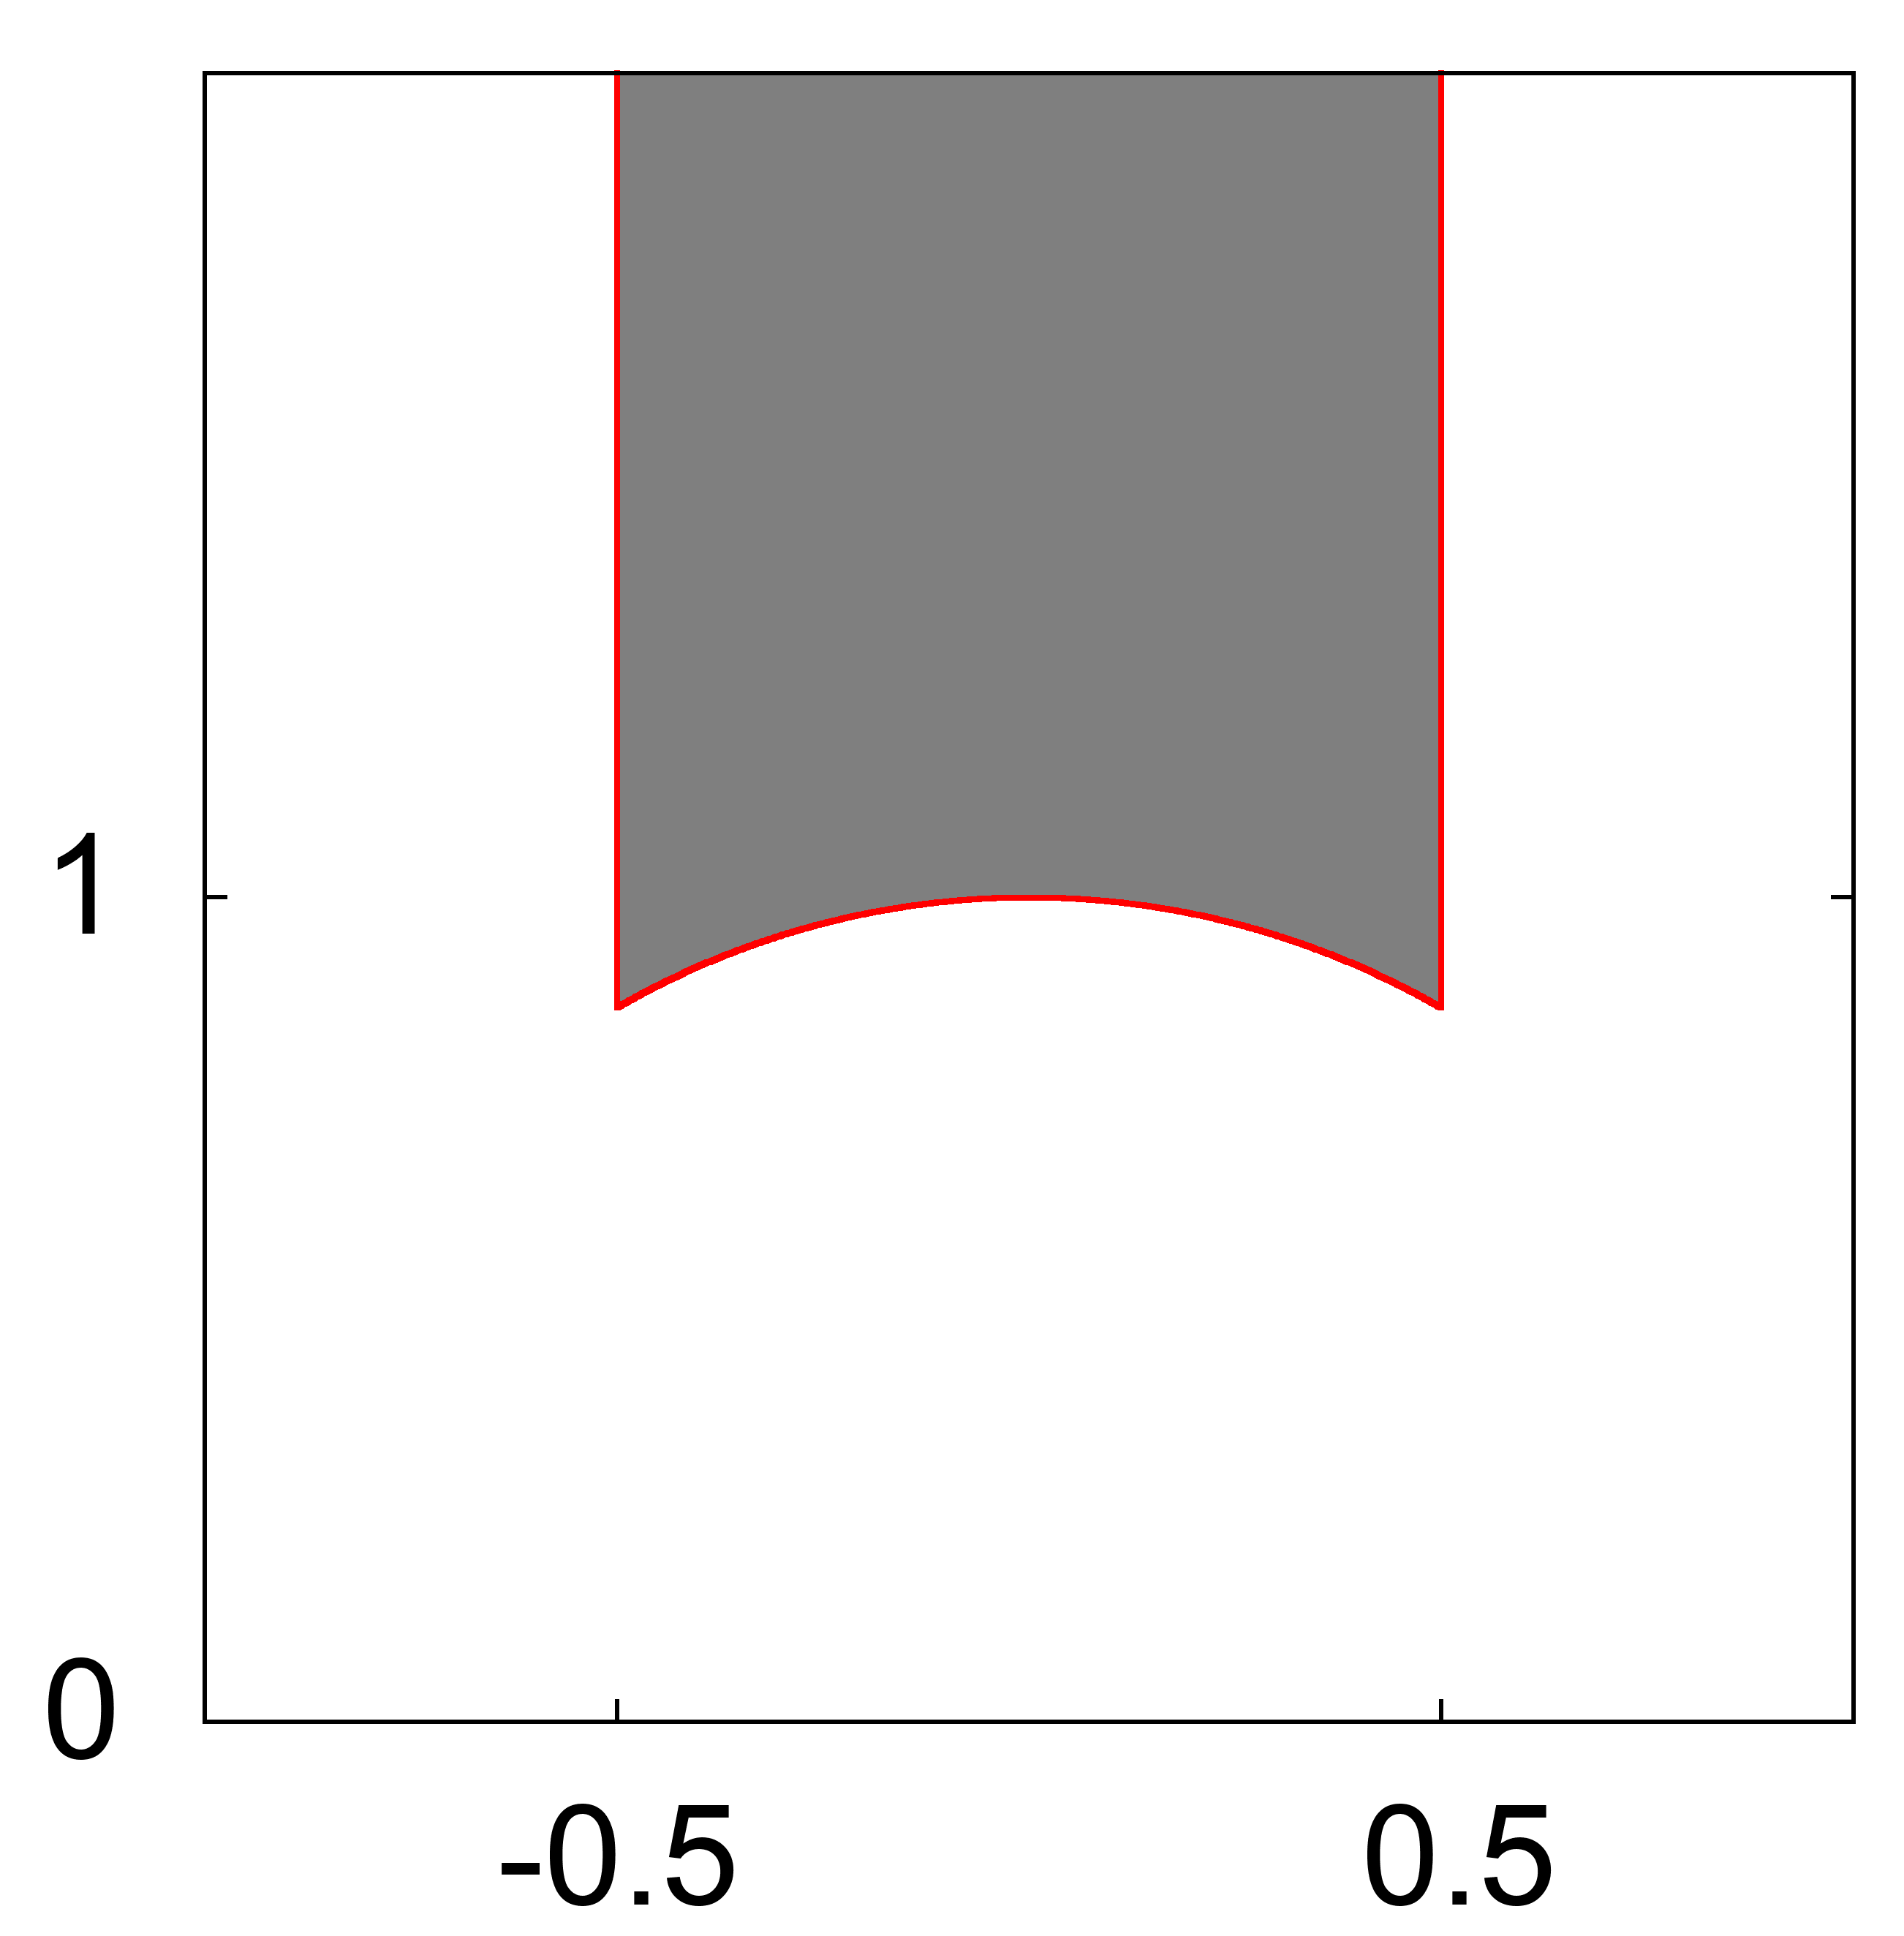
\includegraphics[width=3.5cm]{fd.png}
    \caption{Modular fundamental domain}
  \end{figure}

  We write $\tau = x+yi$ with $x,y\in\IR$ and $y>0$.
  Then $q=e^{-2\pi y} e^{2\pi x}$.
  If $\tau\in \cF$, then $|x|\le 1/2$ and $y\ge \sqrt{3}/2$.
  So $q$ as a function of $(x,y)$ is definable restricted to
  $\cF$. Moreover, $|q|\le e^{-\pi\sqrt{3}}< 1$. Now
  the $q$-expanion of $j$ restricted to the compact ball of radius
  $e^{-\pi\sqrt{3}}$ centered at $0$ is definable in $\IRan$.

  Putting things together we see that $j|_{\cF}\colon
  \cF\rightarrow\IC$ is definable in $\IRanexp$. The restriction is
  surjective.

  Let $m\in\IN$ and consider the product $(\tau_1,\ldots,\tau_m)\mapsto
  (j(\tau_1),\ldots,j(\tau_m))$ which we also denote by
  $j\colon\IH^m\rightarrow\IC^m$. We find that
  $j|_{\cF^m}\colon \cF^m\rightarrow\IC^m=Y(1)(\IC)$ is definable in $\IRanexp$.

  As in Example~\ref{ex:thetafunc} we can consider the preimage of an
  algebraic subvariety $V\subset Y(1)^m$ defined over $\IC$.
  Indeed,
  \begin{equation*}
    j^{-1}(V(\IC)) \cap \cF^m
  \end{equation*}
  is definable in $\IRanexp$ with $\dim j^{-1}(V(\IC))\cap \cF^m =
  2\dim V$.  
\end{example}

\section{Further Reading and Open Problems}

It is known that any function $f \colon \IR\rightarrow\IR$ that is
definable in $\IRan$ is polynomially bounded. That is, there exists
an integer $N\ge 1$ such that $|f(x)|\le x^N$ for all sufficiently
large $x$. This shows that $\exp$ is not definable in $\IRexp$. It is
also known that for any function $f\colon \IR\rightarrow\IR$ that is
definable in $\IRexp$ there exists an $N\ge 1$ such that $|f(x)| \le
\exp^{N}(x)$ for all sufficiently large $x$; here $\exp^{N}$ is the
$N$-fold iterated exponential function. 
Does there exist an o-minimal structure in which a function $f\colon
\IR\rightarrow\IR$ is definable and eventually grows faster than any
finite tower of exponentials?

Further reading:
\begin{itemize}
\item For an overview of o-minimal geometry we refer to the paper of
  van den Dries and Miller~\cite{DM:96}.

\item Theory of theta functions: Mumford's~\cite{MumfordTataLectures}.
\end{itemize}
% \begin{itemize}
% \end{itemize}

%%% Local Variables:
%%% TeX-master: "main"
%%% End:
